% CREATED BY DAVID FRISK, 2015

\chapter{Demo Application}\label{ch_5}
Within the frame of this Thesis, a ``Demo Application'' which is divided in two distinct and independent parts, was created. The system can be tested by following the next link: \url{http://snf-552985.vm.okeanos.grnet.gr/opinion/}.\\
\\
The first part is the ``Back-End'' which is implemented in Java SE8 following the methodology we analysed in Chapter 3, creating in that way, an HTTP server aiming at the communication of these two parts. The second part is the ``Front-End'', which also constitutes the part with which the user communicates with our system, is created with the use of HTML5 and Javascript. These two parts communicate through message exchange in ``JSON'' form. In this demo, the user is given the opportunity to give as ``entry'' a text from the OpenGov  Website.

\centerline{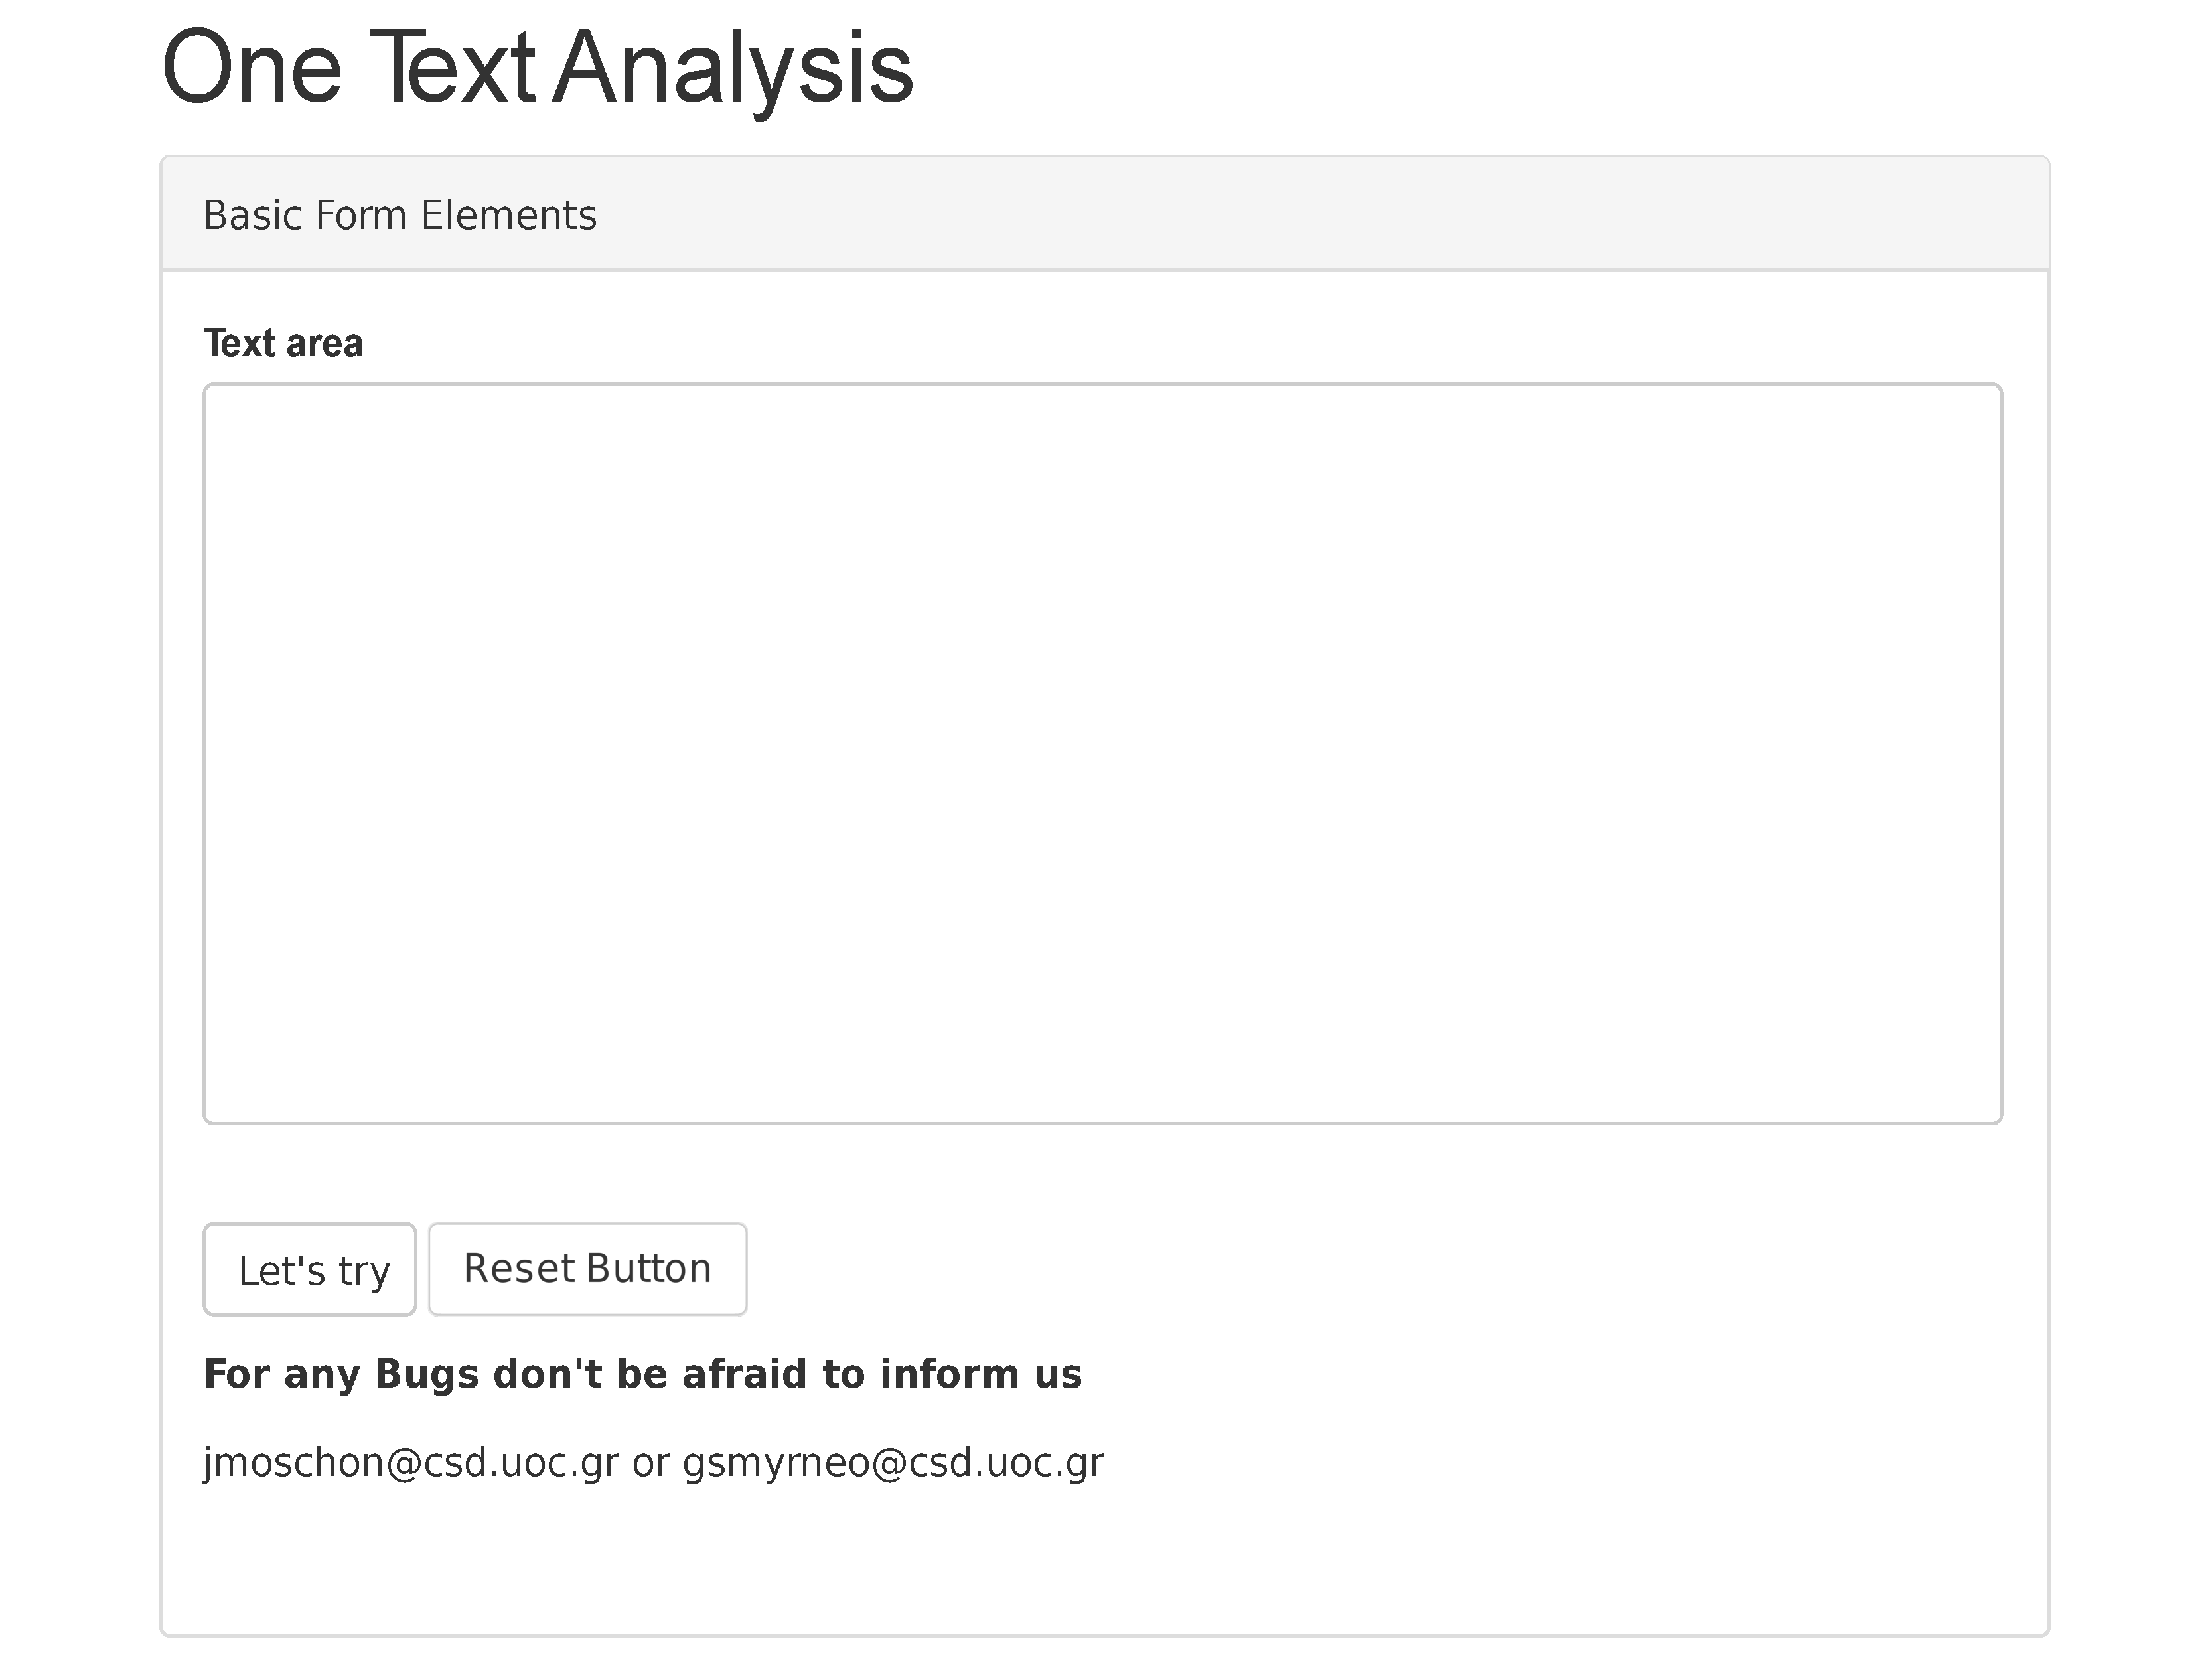
\includegraphics[width=0.85\linewidth]{figure/screens/screen1_vector.pdf}}

In the above picture we can see the initial page in which the user gives the texts that will be analysed.\\
\\

\centerline{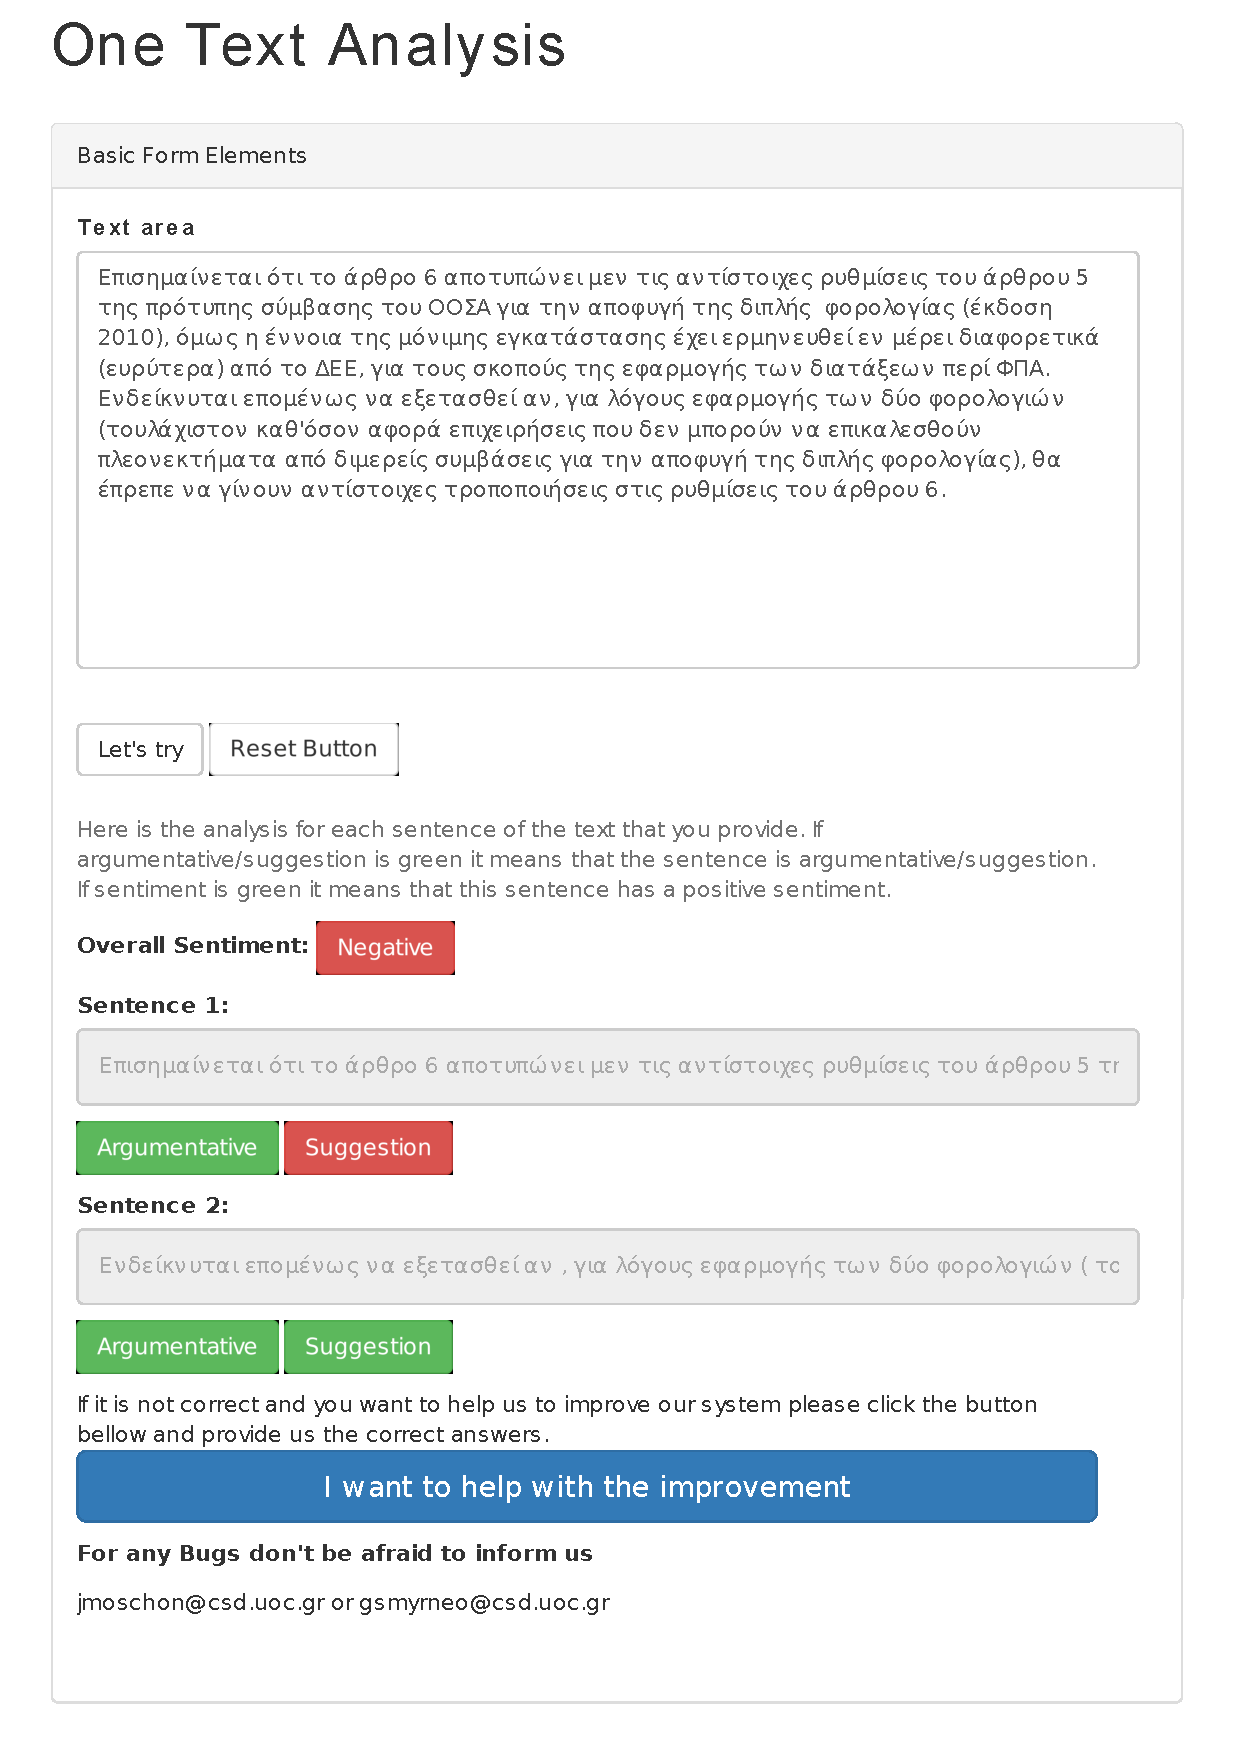
\includegraphics[width=0.9\linewidth]{figure/screens/screen2_vector.pdf}}

By pressing the ``Let's try'' button, the results of the analysis of that specific text appear. The ``Overall Sentiment'' field, is red if the user is negative towards the text and green if he is positive. Then, one by one the sentences of the text appear and below each sentence  an indication whether the sentence is an Argument or a Suggestion and red colour indicates that it is a non-Argument or non-Suggestion.\\
\\
Another useful function that this demo application offers is that the user is being given the chance to ``correct'' that same System in case the results are not correct. This is done by pressing the blue button ``I want to help with the improvement''. We should note that it is an important enough function, because in its total the System is based on Machine Learning.\\
\\

\centerline{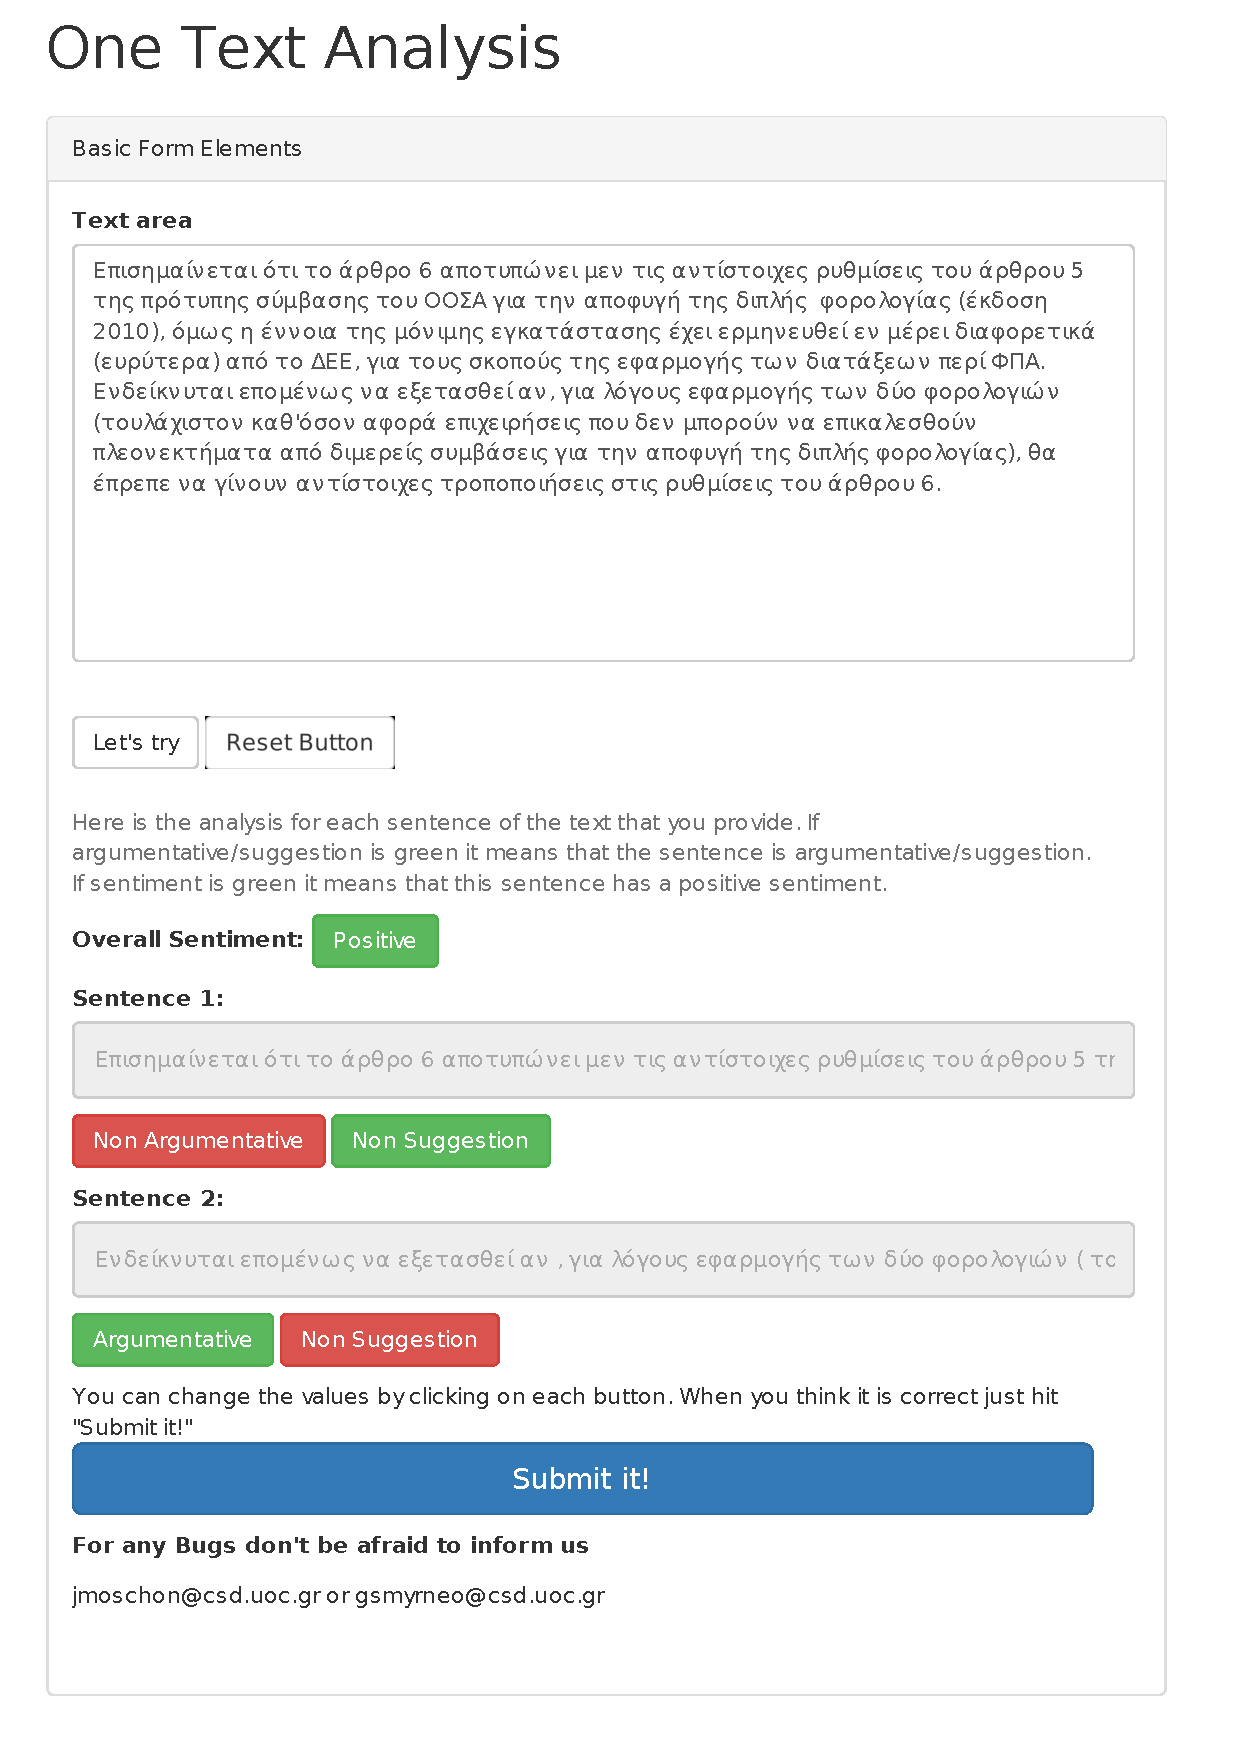
\includegraphics[width=0.9\linewidth]{figure/screens/screen3_vector.pdf}}

After pressing the ``I want to help with the Improvement'' button, as we can see in the above picture the ``characterising'' buttons are now in a deeper colour and the user, by pressing on them can change their colour. When he changes them and considers them to be correct, the next step is to press the ``Submit it'' button in order to send the corrected results back to the System.